\chapter{Frame}\label{frame}

Il laringoscopio fornisce una serie di immagini (detti anche frame) in sequenza che formano un video, non tutti i frame che escono dal laringoscopio sono utili a capire lo stato di salute della laringe di una persona in quanto non sono a fuoco, contengono saliva, riflessi speculari o sono underexposed. Ogni frame contiene una serie una matrice di pixel, se l'immagine è a colori per ogni insieme di pixel sono associati tre colori in codifica RGB (red, green, blue) o HSL/V (hue, saturation, lightness/value) altrimenti a ogni pixel è associato un unico valore, che rappresenta la tonalità di grigio \cite{gonzalez_dip}.

\section{Acquisizione dei frame}\label{acquisizione-dei-frame}

L'acquisizione digitale delle immagini digitalizza solamente lo spettro delle radiazioni elettromagnetiche visibili dall'occhio, detta anche luce, che per comodità, è diviso in sei grandi regioni: viola (0.43 \(\mu \)m), blu, verde, giallo, arancione e rosso (0.79 \(\mu \)m). A differenza del resto del resto dello spettro elettromagnetico, lo spettro della luce non termina bruscamente al variare della lunghezza d'onda, ma invece ogni tonalità di colore si fonde dolcemente con
la successiva tonalità, come mostrato in \cref{fig:spettro-onde} \cite{gonzalez_dip}.

\begin{figure}[ht]
    \centering
    \includegraphics[width=1\textwidth]{frame/Spettro-onde.jpg}
    \caption{Lo spettro elettromagnetico. Lo spettro della luce è mostrato ingrandito}
    \label{fig:spettro-onde}
\end{figure}

La maggior parte delle immagini che ci interessano sono generate dalla combinazione di una o più fonti di illuminazione. A seconda della natura della fonte, l'energia di illuminazione viene riflessa o trasmessa dagli oggetti, come mostrato in \cref{fig:scena-acquisizione} \cite{gonzalez_dip}.

\begin{figure}[ht]
    \centering
    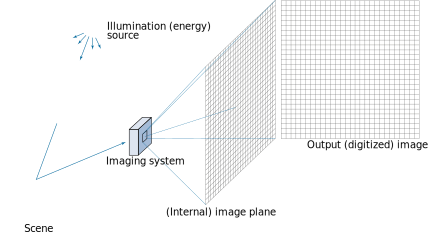
\includegraphics[width=1\textwidth]{frame/digital_image_acquisition.pdf}
    \caption{Esempio di acquisizione di immagini digitali di una scena}
    \label{fig:scena-acquisizione}
\end{figure}

In paticolare una laringoscopia NBI (Narrow binding Imaging)  sfrutta l’emissione una luce bianca a banda stretta assorbita principalmente dall’ emoglobina che permette  di visualizzare la vascolarizzazione delle lesioni laringee e della mucosa circostante \cite{giorgio_cenni_2008}.

\section{Digitalizzazione dei frame}\label{digitalizzazione-dei-frame}

Per la digitalizzazione delle immagini l'idea è semplice: le radiazioni elettromagnetiche  vengono trasformate in una tensione dal sensore, e  viene digitalizzata la forma d'onda in uscita dal sensore, per digitalizzare l'onda è necessario effettuare un campionamento e una quantizzazione, come mostrato in \cref{fig:campionamento-quantizzazione} \cite{gonzalez_dip}.

\begin{figure}[ht]
    \centering
    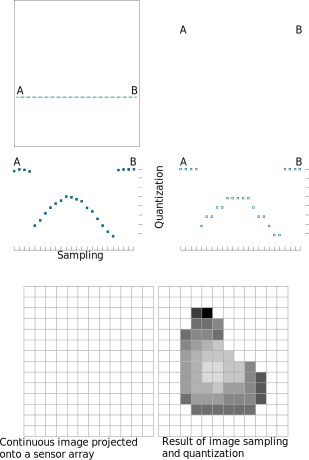
\includegraphics[width=0.5\textwidth]{frame/Sampling-Quantization.pdf}
    \caption{Processo di digitalizzazione di una immagine continua in una digitale}
    \label{fig:campionamento-quantizzazione}
\end{figure}

La relativa rappresenta matematica di una immagine quantizzata è:
\[ f(x, y)=\left[\begin{array}{cccc}f(1,1) & f(1,2) & \cdots & f(1, m) \\ f(2,1) & f(2,2) & \cdots & f(2, m) \\ \vdots & \vdots & & \vdots \\ f(n,1) & f(n,1) & \cdots & f(n,m)\end{array}\right] \]

Dove \(n\times m\) indica la dimensione dell'immagine quantizzata detta anche risoluzione, il valore è determinato in base alla precisione del sensore e se l'immagine ha subito post elaborazioni, come un crop. In particolare si definisce pixel  (o anche dot) ogni elemento dell'immagine quantizzata \(f(x, y)\). Si definisce raster la griglia ortogonale di pixel che costituisce una immagine. Il pixel può essere un unico valore scalare che quindi rappresenta una scala di grigi oppure essere un array di 3 scalari che indicano le tonalità di colore, come mostrato nella figura \cref{fig:rgb-raster-image}. In notazione matematica il numero di canali di colore viene spesso aggiunto alla risoluzione nel seguente formato: \(n\times m \times c\) ottenendo quindi una matrice a più dimensioni, detta anche tensore \cite{gonzalez_dip}. La relativa rappresenta matematica di una immagine quantizzata a colori con codifica RGB è:

\begin{figure}[ht]
    \centering
    \tdplotsetmaincoords{75}{20}
    \begin{tikzpicture}[tdplot_main_coords]
        \begin{scope}[canvas is xz plane at y=2,transform shape]
            \node[inner sep=0pt,text=blue,opacity=0.8] (mat1)
            {\(\displaystyle\begin{bmatrix*}[c]
                    f_b(1,1) & f_b(1,2) & \cdots & f_b(1, m) \\ f_b(2,1) & f_b(2,2) & \cdots & f_b(2, m) \\ \vdots & \vdots & & \vdots \\ f_b(n,1) & f_b(n,1) & \cdots & f_b(n,m) \\
                \end{bmatrix*}\)};

            \begin{scope}[on background layer]
                \fill[blue,opacity=0.2] (mat1.south west) coordinate (blb) -- (mat1.south east) coordinate (brb) -- (mat1.north  east) coordinate (trb) -- (mat1.north  west) coordinate (tlb);
            \end{scope}
        \end{scope}
        %
        \begin{scope}[canvas is xz plane at y=0,transform shape]
            \node[inner sep=0pt,text=green!70!black,opacity=0.8] (mat2) {\(\displaystyle
                \begin{bmatrix*}[c]
                    f_g(1,1) & f_g(1,2) & \cdots & f_g(1, m) \\ f_g(2,1) & f_g(2,2) & \cdots & f_g(2, m) \\ \vdots & \vdots & & \vdots \\ f_g(n,1) & f_g(n,1) & \cdots & f_g(n,m) \\
                \end{bmatrix*}\)};

            \begin{scope}[on background layer]
                \fill[green!70!black,opacity=0.2] (mat2.south west) coordinate (blb) -- (mat2.south east) coordinate (brb) -- (mat2.north  east) coordinate (trb) -- (mat2.north  west) coordinate (tlb);
            \end{scope}
        \end{scope}
        %
        \begin{scope}[canvas is xz plane at y=-2,transform shape]
            \node[inner sep=0pt,text=red,opacity=0.8] (mat3) {\(\displaystyle
                \begin{bmatrix*}[c]
                    f_r(1,1) & f_r(1,2) & \cdots & f_r(1, m) \\ f_r(2,1) & f_r(2,2) & \cdots & f_r(2, m) \\ \vdots & \vdots & & \vdots \\ f_r(n,1) & f_r(n,1) & \cdots & f_r(n,m) \\
                \end{bmatrix*}\)};

            \begin{scope}[on background layer]
                \fill[red,opacity=0.2]
                (mat3.south west) coordinate (blb) -- (mat3.south east) coordinate (brb) -- (mat3.north  east) coordinate (trb) -- (mat3.north  west) coordinate (tlb);
            \end{scope}
        \end{scope}
        %\foreach \X in {tl,tr,br}
        %{\draw[thin,orange] (\X f) -- (\X b);}
        %\begin{scope}[on background layer]
        % \draw[thin,orange] (blf) -- (blb);
        %\end{scope}
        \node[left] at (mat2.west) {\(f(x,y,k)=\quad \quad\)};
    \end{tikzpicture}
\end{figure}

\begin{figure}[ht]
    \centering
    \includegraphics[width=0.27\textwidth]{frame/Rgb-raster-image.pdf}
    \caption{Immagine raster RGB}
    \label{fig:rgb-raster-image}
\end{figure}

Intuitivamente la risoluzione indica la  misura del più piccolo dettaglio distinguibile in una immagine. Quantitativamente la risoluzione può essere espressa in diversi modi, dal più semplice \(n\times m\) ad unità più complesse come il dpi (dots per inch), che indica quanti pixel ci sono in una unità di distanza. La risoluzione influisce molto sulla qualità dell'immagine, in \cref{fig:resolution-on-image-quality} è presente la stessa immagine campionata con una risoluzione diversa \cite{gonzalez_dip} \cite{spaepen_resolution}.

\begin{figure}[ht]
    \centering
    \includegraphics[width=0.5\textwidth]{frame/resolution-on-image-quality.png}
    \caption{Effetto della risoluzione sulla qualità dell'immagine}
    \label{fig:resolution-on-image-quality}
\end{figure}

Oltre alla risoluzione c'è un altro fattore che indica la qualità dell'immagine, dato che l'immagine è una informazione di tipo continuo, ma in un computer è possibile rappresentare solamente informazioni quantizzate a dimensione finita è necessario definire un numero di bit per canale, questo valore moltiplicato per la risoluzione e il numero di canali dell'immagine  \(n\times m \times d\) fornisce la dimensione in bit dell'immagine raster non compressa. L'uso di un numero di bit per canale  troppo basso porta ad una perdita di risoluzione, come mostrato in \cref{fig:bit-channel}  \cite{gonzalez_dip} \cite{spaepen_resolution}.

\begin{figure}[ht]
    \centering
    \includegraphics[width=0.5\textwidth]{frame/bit-channel.png}
    \caption{Effetto del numero di bit per canale sulla qualità dell'immagine}
    \label{fig:bit-channel}
\end{figure}